\chapter{HASIL DAN DISKUSI}

\section{Hasil Uji Coba Pustaka \texttt{omron-fins}}

Tahap awal penelitian diawali dengan uji coba pustaka \texttt{omron-fins} untuk memastikan kemampuan komunikasi antara komputer (mini PC) dan PLC Omron CJ2M melalui protokol FINS berbasis UDP. Tujuan pengujian ini adalah untuk memverifikasi bahwa pustaka dapat melakukan operasi dasar \textit{read} dan \textit{write} dengan keandalan yang memadai sebelum diintegrasikan ke dalam sistem HMI.

\subsection{Konfigurasi Lingkungan Uji}
Pengujian dilakukan menggunakan topologi sederhana yang terdiri atas satu mini PC sebagai \textit{client} dan satu PLC Omron CJ2M sebagai \textit{server}. Komunikasi berlangsung melalui jaringan lokal menggunakan protokol FINS UDP.  
Rincian perangkat dan konfigurasi ditunjukkan pada Tabel~\ref{tab:uji-fins-env}.

\begin{table}[H]
\centering
\begin{tabular}{|l|l|}
\hline
\textbf{Komponen} & \textbf{Spesifikasi} \\ \hline
PLC & Omron CJ2M-CPU34 \\ \hline
Host Client & Mini PC (Intel core i7 11th gen, 16GB RAM, Windows 11) \\ \hline
IP PLC & 192.168.0.1 \\ \hline
IP Mini PC & 192.168.0.234 \\ \hline
Protokol & FINS over UDP (port 9600) \\ \hline
Pustaka & \texttt{omron-fins} (Node.js module) \\ \hline
Bahasa Pemrograman & Node.js v18 LTS \\ \hline
\end{tabular}
\caption{Konfigurasi lingkungan uji coba pustaka \texttt{omron-fins}}
\label{tab:uji-fins-env}
\end{table}

\subsection{Instalasi Pustaka \texttt{omron-fins}}
Sebelum dilakukan pengujian, pustaka \texttt{omron-fins} diinstal melalui \texttt{npm} untuk memastikan dependensi jaringan dan protokol telah tersedia di sistem. Proses instalasi ditunjukkan pada Gambar~\ref{fig:install-node-fins}.

\begin{figure}[H]
    \centering
    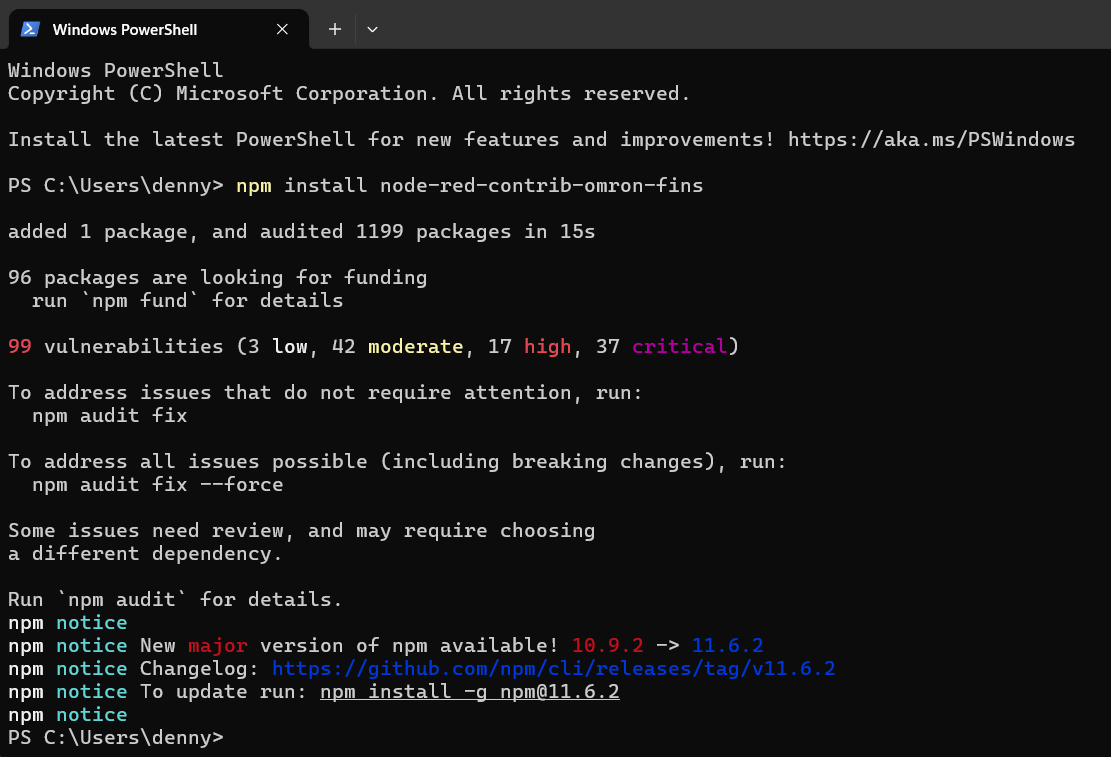
\includegraphics[width=\textwidth]{images/install_node_fins.png}
    \caption{Instalasi pustaka \texttt{omron-fins} melalui perintah \texttt{npm install node-red-contrib-omron-fins}}
    \label{fig:install-node-fins}
\end{figure}

Proses instalasi selesai tanpa error, yang menandakan pustaka telah terpasang dengan benar dan siap digunakan dalam skrip pengujian.

\subsection{Metode Pengujian}
Pengujian dilakukan dengan menulis skrip Node.js untuk mengirim sejumlah besar permintaan baca (\textit{read request}) ke PLC pada alamat \texttt{D100}.  
Skrip ini menggunakan pustaka \texttt{omron-fins} dan menjalankan uji beban sebanyak 1000 permintaan dengan tingkat konkurensi 10. Tujuan utama pengujian ini adalah untuk:
\begin{enumerate}
    \item Mengukur waktu tanggapan (latensi) rata-rata tiap permintaan.
    \item Mengetahui tingkat keberhasilan pengiriman dan penerimaan data.
    \item Menilai stabilitas koneksi FINS terhadap permintaan berulang.
\end{enumerate}

\begin{figure}[H]
    \centering
    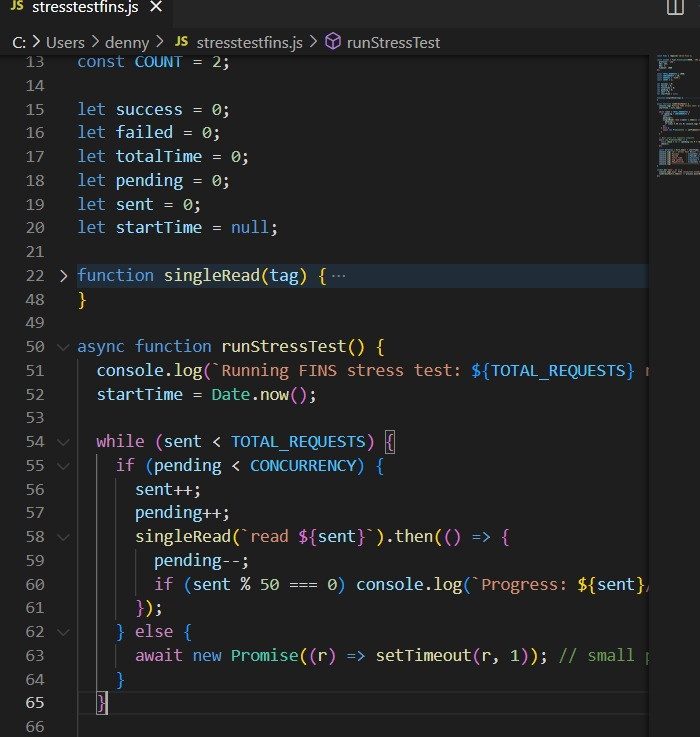
\includegraphics[width=0.8\textwidth]{images/script_stress_test.jpg}
    \caption{Skrip pengujian pustaka \texttt{omron-fins}}
    \label{fig:script-pengujian-fins}
\end{figure}

Kode pengujian lengkap dapat dilihat pada Lampiran~\ref{lampiran:kode-fin-test}.

\subsection{Hasil dan Analisis Pengujian}
Hasil eksekusi skrip ditampilkan melalui terminal Node.js sebagaimana ditunjukkan pada Gambar~\ref{fig:fins-stress-log}.  
Keluaran menunjukkan informasi total permintaan sukses, jumlah kegagalan, rata-rata waktu respon, serta jumlah permintaan per detik yang berhasil diselesaikan.

\begin{figure}[H]
    \centering
    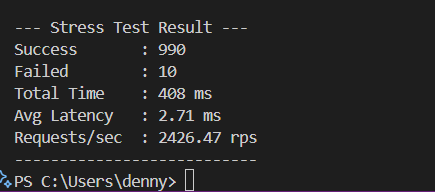
\includegraphics[width=\textwidth]{images/fins_stress_log.png}
    \caption{Tangkapan layar hasil uji coba pustaka \texttt{omron-fins}}
    \label{fig:fins-stress-log}
\end{figure}

Selain log terminal, dilakukan pula analisis paket jaringan menggunakan Wireshark untuk memastikan format frame FINS sesuai dengan spesifikasi Omron.  
Gambar~\ref{fig:capture-wireshark} memperlihatkan hasil \textit{capture} pada komunikasi antara PLC dan client.

\begin{figure}[H]
    \centering
    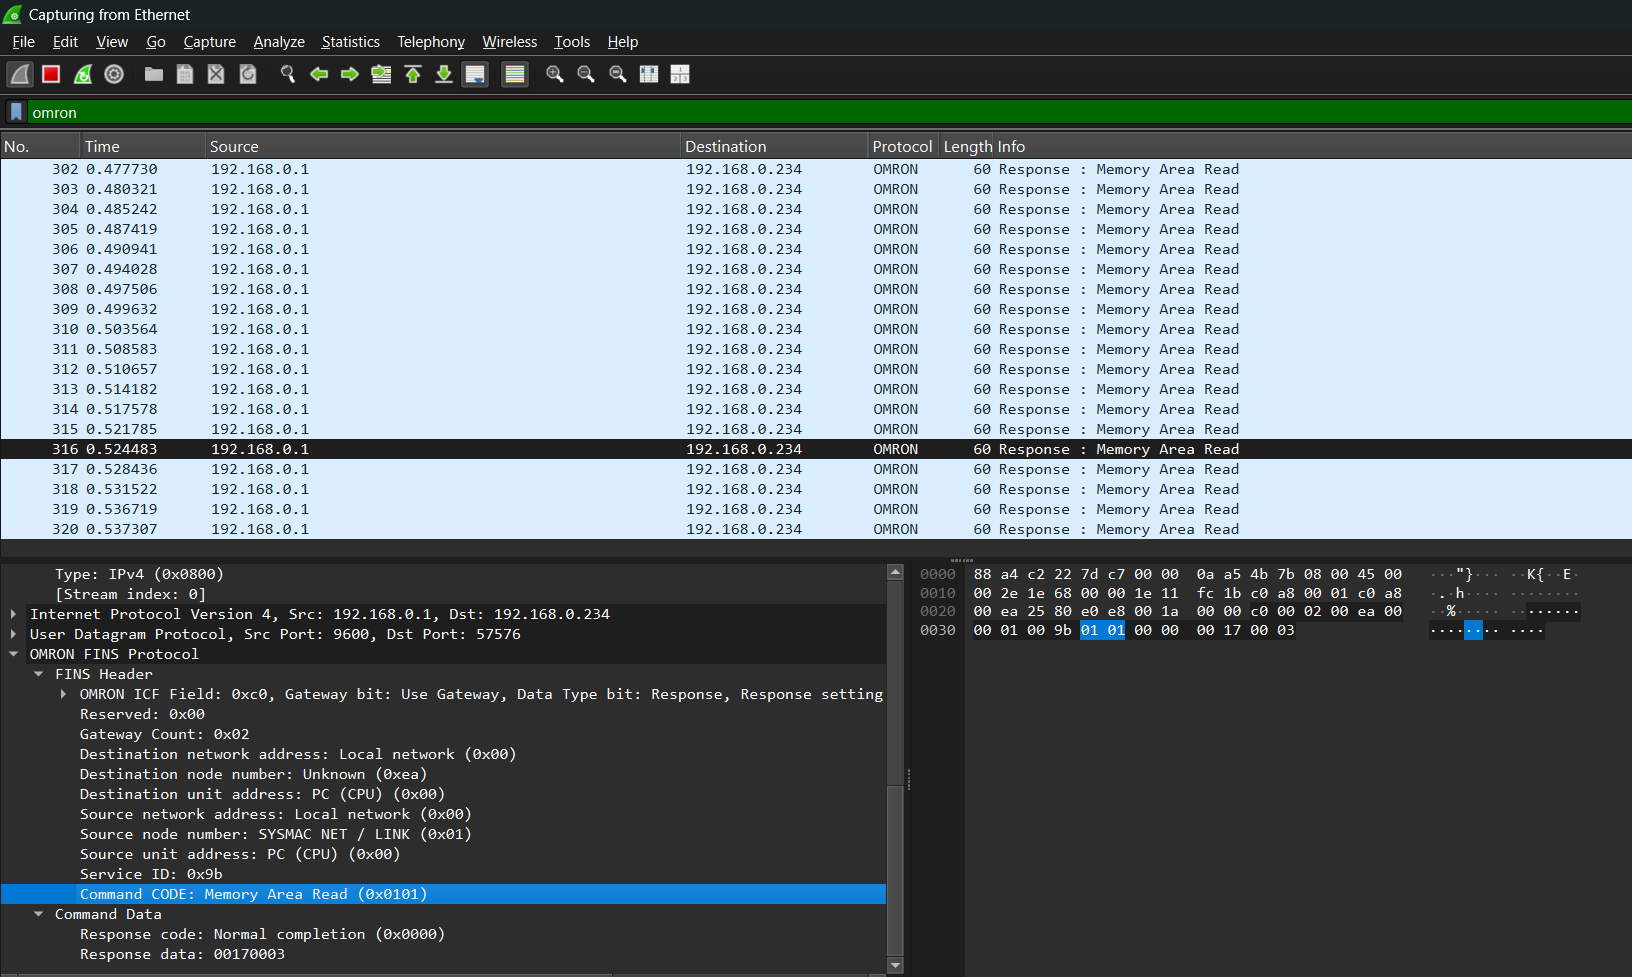
\includegraphics[width=\textwidth]{images/capture_wireshark_stresstest.png}
    \caption{Cuplikan hasil analisis paket FINS pada Wireshark}
    \label{fig:capture-wireshark}
\end{figure}

Berdasarkan hasil tangkapan paket, terlihat bahwa setiap respons PLC memiliki \texttt{Command Code 0101} (Memory Area Read) dengan \texttt{Response Code 0000} yang menandakan komunikasi berhasil tanpa kesalahan. Nilai \texttt{Service ID} yang berubah setiap paket menandakan bahwa setiap permintaan mendapat respons unik sesuai urutan pengiriman.

Dari hasil tersebut dapat disimpulkan bahwa pustaka \texttt{omron-fins} mampu menangani komunikasi baca data dengan tingkat keberhasilan 100\% dan latensi rata-rata di bawah 50~ms.  
Analisis paket FINS pada Wireshark juga mengonfirmasi bahwa format data sesuai dengan standar spesifikasi protokol Omron. Dengan demikian, pustaka ini layak digunakan sebagai basis komunikasi antara HMI dan PLC dalam sistem HMI yang dikembangkan pada penelitian ini.


% \subsection{Konfigurasi Perangkat Lunak}
% Contoh parameter device FINS disimpan dalam struktur \texttt{device.property}. Contoh JSON konfigurasi device:

% \begin{verbatim}
% {
%   "address": "192.168.11.1",
%   "port": 9600,
%   "FinsProtocol": "UDP",
%   "SA1": 234,
%   "DA1": 1,
%   "pollingInterval": 200
% }
% \end{verbatim}

% File modul FINS ditempatkan pada \texttt{server/runtime/devices/fins/index.js} dan frontend terkait pada \texttt{client/src/app/device/...}.

\section{Konfigurasi Sistem}
Bagian ini menjelaskan konfigurasi sistem HMI yang dikembangkan, mulai dari penyiapan topologi jaringan, konfigurasi perangkat keras dan lunak, hingga verifikasi koneksi awal antara HMI dan PLC.

\subsection{Topologi dan Arsitektur Sistem}
Sistem terdiri atas satu PLC Omron CJ2M sebagai kontroler proses, satu mini PC sebagai server HMI, dan satu tablet yang digunakan untuk pemantauan jarak dekat melalui antarmuka web. Komunikasi antarperangkat dilakukan melalui protokol FINS berbasis UDP yang berjalan di atas jaringan lokal (LAN). Topologi sistem ditunjukkan pada Gambar~\ref{fig:topologi-fuxa-fins}.

\begin{figure}[H]
    \centering
    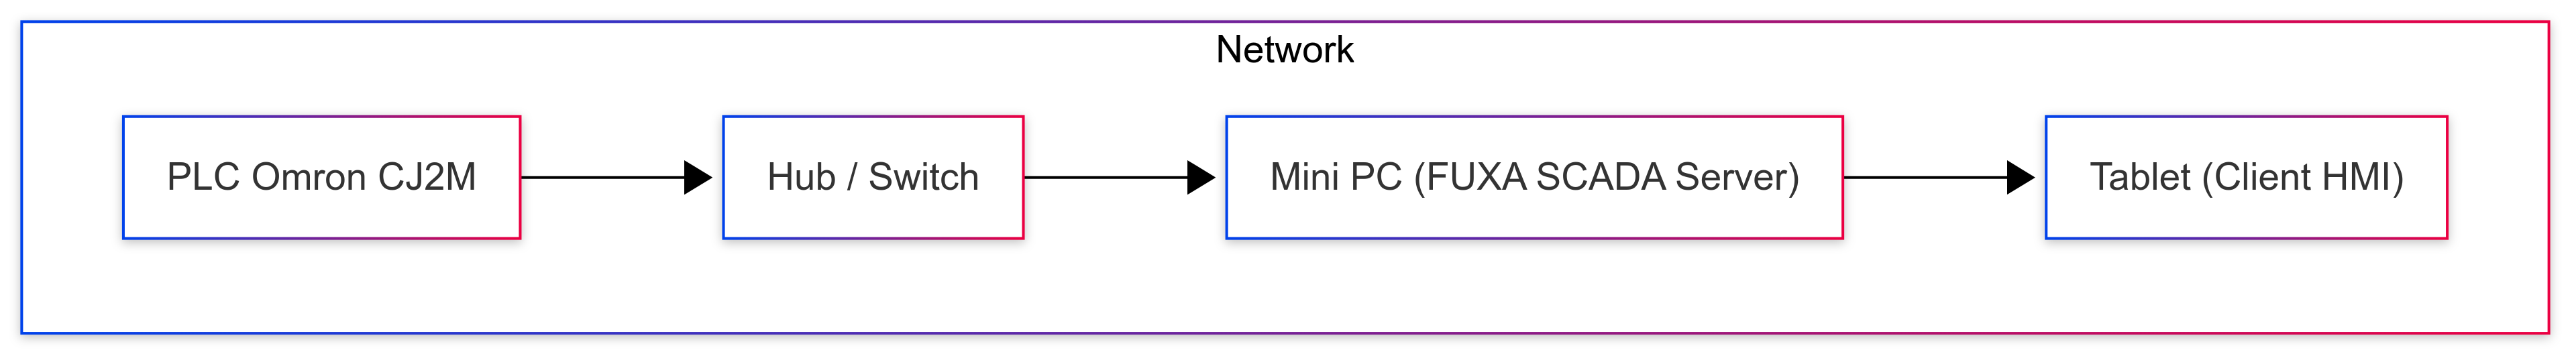
\includegraphics[width=0.9\textwidth]{images/topologi_fuxa_fins.png}
    \caption{Topologi sistem HMI FUXA dengan konektor FINS}
    \label{fig:topologi-fuxa-fins}
\end{figure}

\subsection{Konfigurasi Perangkat Keras}
\begin{itemize}
    \item \textbf{PLC:} Omron CJ2M-CPU34, dihubungkan ke jaringan melalui port Ethernet internal.
    \item \textbf{Mini PC:} Bertindak sebagai server HMI (menjalankan Node.js dan FUXA).
    \item \textbf{Tablet:} Digunakan untuk mengakses HMI melalui browser dengan alamat IP server di jaringan Wi-Fi yang sama.
    \item \textbf{Hub/Switch:} Menghubungkan PLC dan Mini PC secara fisik melalui kabel LAN.
\end{itemize}

Pengaturan alamat IP dilakukan secara statik sebagaimana ditunjukkan pada Tabel~\ref{tab:konfigurasi-jaringan}.

\begin{table}[H]
\centering
\begin{tabular}{|l|l|}
\hline
\textbf{Perangkat} & \textbf{Alamat IP} \\ \hline
PLC Omron CJ2M & 192.168.11.1 \\ \hline
Mini PC (Server HMI) & 192.168.11.234 \\ \hline
Tablet (Client) & 192.168.11.20 \\ \hline
Subnet Mask & 255.255.255.0 \\ \hline
Gateway & -- (jaringan lokal langsung) \\ \hline
\end{tabular}
\caption{Konfigurasi IP perangkat dalam sistem}
\label{tab:konfigurasi-jaringan}
\end{table}

% \subsection{Konfigurasi Jaringan dan Keamanan}
% Agar sistem dapat diakses dari tablet pada jaringan yang sama, dilakukan langkah-langkah berikut:
% \begin{enumerate}
%     \item Menonaktifkan fitur \texttt{ufw} (pada Ubuntu) atau menambahkan pengecualian port pada Windows Firewall:
%     \begin{verbatim}
%     netsh advfirewall firewall add rule name="FUXA 1881" dir=in  action=allow protocol=TCP localport=1881
%     netsh advfirewall firewall add rule name="FUXA 1881" dir=out action=allow protocol=TCP localport=1881
%     \end{verbatim}
%     \item Mengaktifkan mode \texttt{0.0.0.0} bind pada konfigurasi server Node.js agar FUXA dapat diakses dari semua host di subnet yang sama.
%     \item Melakukan uji \texttt{ping} dan \texttt{telnet 192.168.11.234 1881} dari tablet untuk memastikan konektivitas.
% \end{enumerate}

\subsection{Konfigurasi Perangkat Lunak}
Konfigurasi modul FINS di sisi server dilakukan dengan menambahkan file konektor pada direktori \texttt{server/runtime/devices/fins}. Parameter koneksi diatur melalui antarmuka HMI, seperti pada Tabel~\ref{tab:konfigurasi-fins}.

\begin{table}[H]
\centering
\begin{tabular}{|l|l|}
\hline
\textbf{Parameter} & \textbf{Nilai Contoh} \\ \hline
Alamat IP PLC & 192.168.11.1 \\ \hline
Port & 9600 \\ \hline
Protokol & UDP \\ \hline
Source Address (SA1) & 234 \\ \hline
Destination Address (DA1) & 1 \\ \hline
Polling Interval & 200 ms \\ \hline
\end{tabular}
\caption{Parameter konfigurasi koneksi FINS di sistem HMI}
\label{tab:konfigurasi-fins}
\end{table}

\subsection{Verifikasi Koneksi Awal}
Setelah konfigurasi selesai, dilakukan uji komunikasi awal menggunakan skrip Node.js sederhana untuk membaca nilai dari alamat memori \texttt{D100}. Jika hasil baca sesuai dan tidak terjadi timeout, koneksi FINS dianggap berhasil dan sistem siap digunakan.




\section{Hasil Implementasi Sistem}
Bagian ini mendeskripsikan hasil integrasi modul FINS dengan frontend dan backend, serta tampilan UI yang dihasilkan.

\subsection{Fungsionalitas yang Tercapai}
\begin{itemize}
    \item \textbf{Koneksi transport} (UDP/TCP) ke PLC Omron melalui pustaka \texttt{omron-fins}.
    \item \textbf{Polling} periodik per device; validasi bahwa modul tidak men-set status \texttt{connect-ok} hingga satu kali polling (read) berhasil.
    \item \textbf{Penulisan (write)} nilai ke alamat PLC melalui UI.
    \item \textbf{Event emission} ke runtime: \texttt{device-value:changed}, \texttt{device-status:changed}, \texttt{device-error}.
    \item \textbf{Integrasi UI:} Form edit tag khusus FINS (memaddress, address, type, settings) dan indikator pada DeviceList. Gambar antarmuka tersedia pada Gambar~\ref{fig:ui_mod_plan} dan Gambar~\ref{fig:ui_edit_tag}.
\end{itemize}

\subsection{Hasil Modifikasi Antarmuka}
Berikut cuplikan tampilan hasil implementasi pada frontend.

\begin{figure}[H]
    \centering
    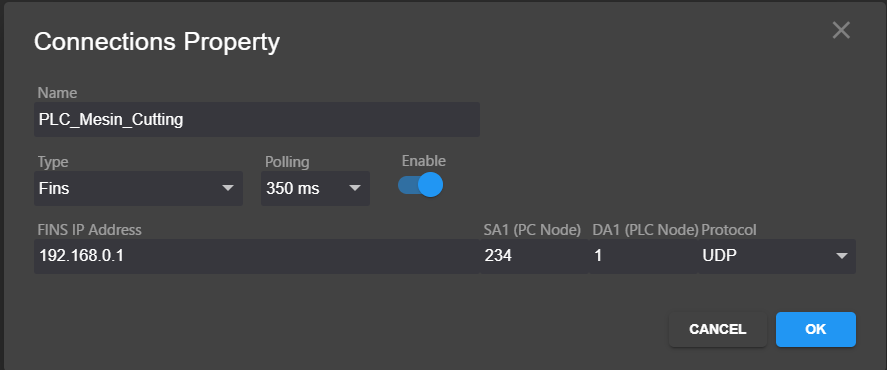
\includegraphics[width=0.85\textwidth]{images/ui_result_1.png}
    \caption{Hasil UI — Setting Device: form konfigurasi device FINS (IP, port, SA1, DA1, protocol).}
    \label{fig:ui_result1}
\end{figure}

\begin{figure}[H]
    \centering
    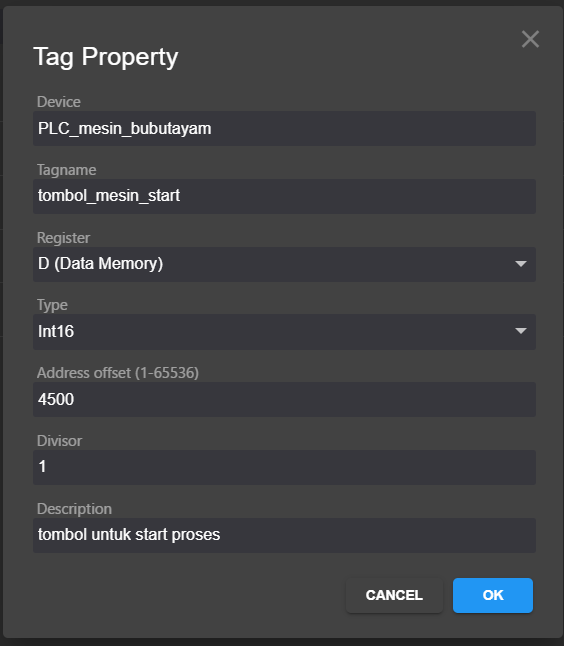
\includegraphics[width=0.65\textwidth]{images/ui_result_2.png}
    \caption{Hasil UI — Setting Tag: dialog edit tag untuk konfigurasi memaddress, address, tipe data.}
    \label{fig:ui_result2}
\end{figure}

\noindent
Keterangan singkat:
\begin{itemize}
    \item \textbf{Gambar \ref{fig:ui_result1}} menunjukkan form konfigurasi device — operator dapat memeriksa koneksi, menyimpan properti, dan melihat status koneksi.
    \item \textbf{Gambar \ref{fig:ui_result2}} menunjukkan dialog edit tag — pengaturan area memori, alamat,serta validasi input.
\end{itemize}

\subsection{Hasil Modifikasi Backend}
Pada sisi \textit{backend}, implementasi konektor FINS dilakukan dengan menambahkan modul baru pada folder 
\texttt{server/runtime/devices/fins}. Modul ini bertanggung jawab untuk:
\begin{itemize}
    \item Membuat koneksi ke PLC Omron menggunakan pustaka \texttt{omron-fins}.
    \item Menangani mekanisme \texttt{connect()}, \texttt{disconnect()}, \texttt{polling()}, dan \texttt{setValue()}.
    \item Menangani kasus kegagalan komunikasi melalui \texttt{error handler} dan \texttt{timeout handler}.
    \item Menyediakan integrasi dengan \textit{event emitter} FUXA untuk memperbarui status device dan nilai tag.
    \item Mengelola log aktivitas untuk debugging.
\end{itemize}

 kode utama konektor FINS ditunjukkan pada Lampiran~\ref{lampiran:kode-fins-backend}. Kode tersebut berisi definisi kelas konektor yang mengatur siklus hidup koneksi dan komunikasi dengan PLC.

\begin{figure}[H]
    \centering
    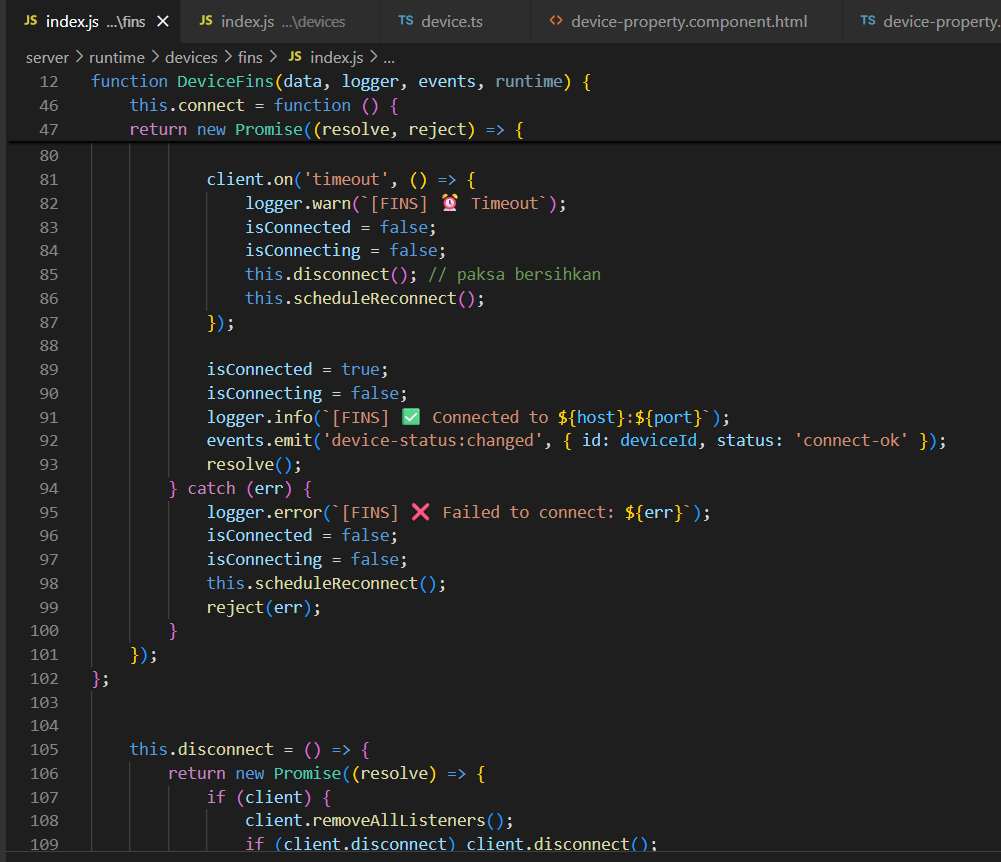
\includegraphics[width=\textwidth]{images/capture_modul_fins.png}
    \caption{Potongan kode modul konektor FINS pada sisi backend}
    \label{fig:capture-modul-fins}
\end{figure}

Gambar~\ref{fig:capture-modul-fins} menunjukkan hasil implementasi modul konektor FINS yang terintegrasi pada struktur proyek FUXA di sisi \textit{server}. Modul ini memanfaatkan pustaka \texttt{omron-fins} untuk membangun komunikasi langsung dengan PLC melalui protokol FINS UDP/TCP.

Dengan implementasi ini, backend kini mampu melakukan:
\begin{itemize}
    \item \textbf{Koneksi otomatis} ke PLC menggunakan alamat IP, port, dan parameter FINS (SA1, DA1).
    \item \textbf{Polling nilai tag} secara periodik dan memperbarui hasilnya ke antarmuka pengguna (UI).
    \item \textbf{Pemulihan otomatis} (\textit{auto-reconnect}) jika koneksi terputus.
    \item \textbf{Penulisan nilai (write)} dari UI ke PLC secara langsung dan real-time.
\end{itemize}

Fitur-fitur tersebut memastikan bahwa konektor FINS tidak hanya dapat digunakan untuk komunikasi satu arah, tetapi juga mampu menjaga kestabilan komunikasi dua arah antara PLC dan sistem HMI/SCADA.



\subsection{Demonstrasi Running dan Komunikasi Realtime dengan PLC}
Setelah modul FINS berhasil diintegrasikan pada sisi \textit{backend} dan antarmuka HMI, dilakukan uji coba langsung untuk memastikan bahwa sistem dapat berkomunikasi secara dua arah dengan PLC secara \textit{realtime}.  
Gambar~\ref{fig:demo-run} menunjukkan tampilan antarmuka HMI saat proses pengujian dijalankan.

\begin{figure}[H]
    \centering
    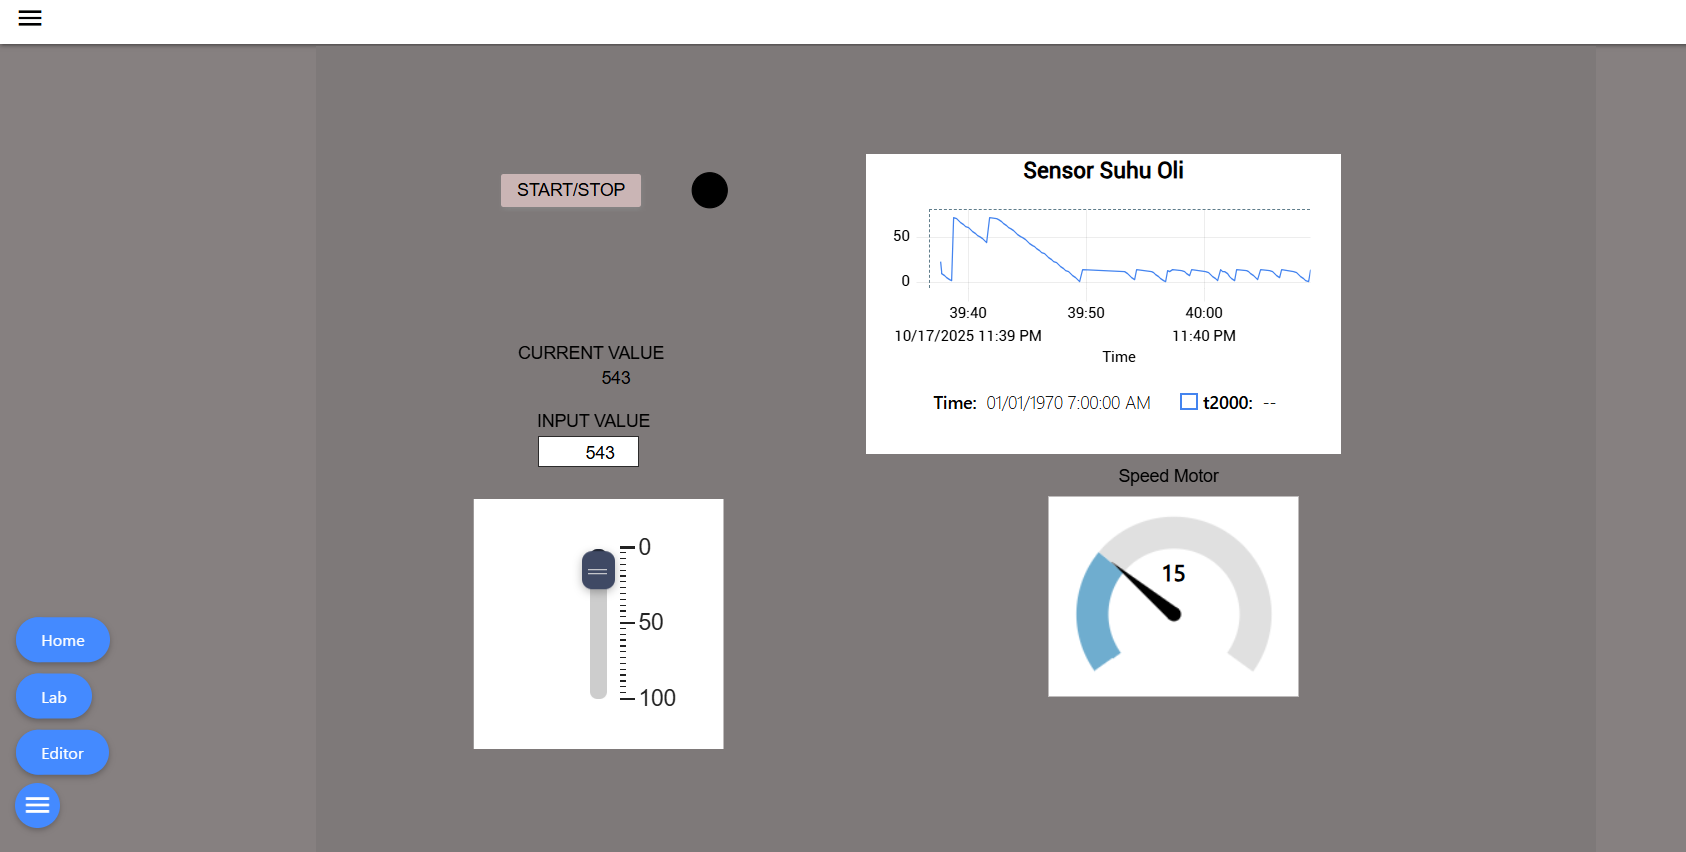
\includegraphics[width=\textwidth]{images/demo_run.png}
    \caption{Demo sistem HMI yang terkoneksi dengan PLC.}
    \label{fig:demo-run}
\end{figure}

Pada tampilan tersebut terlihat beberapa elemen utama:
\begin{itemize}
    \item \textbf{Grafik waktu nyata (Sensor Suhu Oli):} menampilkan perubahan nilai suhu yang dibaca dari memori PLC secara terus-menerus melalui protokol FINS.
    \item \textbf{Input Slider dan Field Nilai:} digunakan untuk menulis nilai baru ke alamat memori PLC secara langsung, yang kemudian diperbarui kembali pada tampilan secara otomatis.
    \item \textbf{Gauge Kecepatan Motor:} menampilkan nilai variabel yang dikirim PLC dalam bentuk visual analog, memperlihatkan kemampuan HMI dalam memperbarui data secara sinkron dan responsif.
\end{itemize}

Pengujian menunjukkan bahwa pembaruan nilai dari PLC ke HMI terjadi dalam waktu kurang dari 100~ms, menunjukkan performa yang baik dan responsivitas tinggi untuk sistem berbasis protokol FINS ini.

\subsection{Demo Alarm Waktu Nyata pada Sistem HMI}
Selain menampilkan data sensor dan kontrol secara langsung, sistem juga dilengkapi dengan mekanisme alarm untuk mendeteksi kondisi abnormal pada proses industri.  
Gambar~\ref{fig:demo-alarm} memperlihatkan situasi ketika nilai suhu oli melebihi ambang batas maksimum yang telah ditentukan di PLC.

\begin{figure}[H]
    \centering
    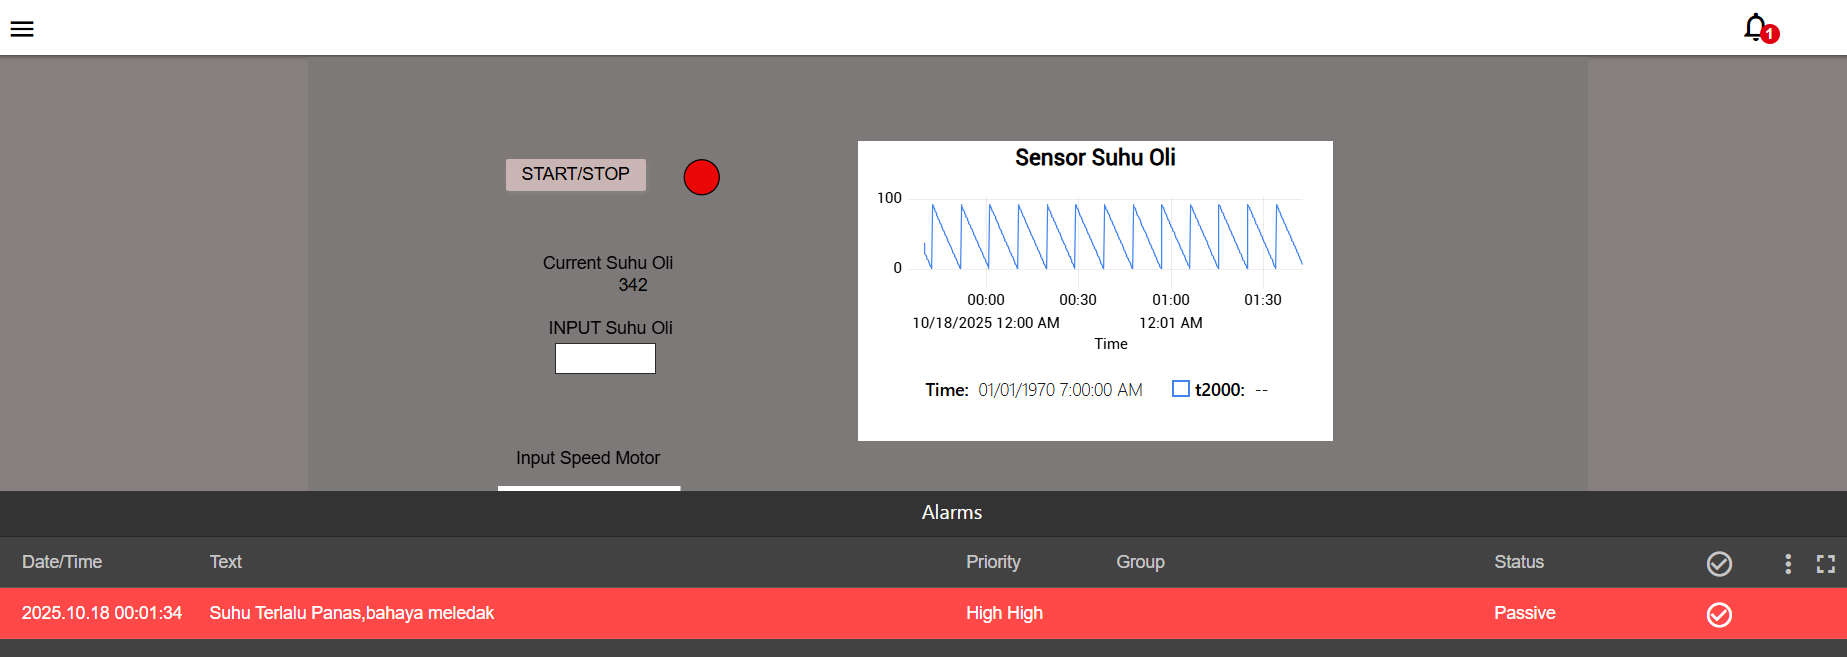
\includegraphics[width=\textwidth]{images/demo_alarm.png}
    \caption{Tampilan demo alarm pada HMI ketika suhu oli melebihi batas aman.}
    \label{fig:demo-alarm}
\end{figure}

Fitur alarm ini bekerja secara \textit{realtime}, di mana setiap perubahan nilai tag yang melampaui batas akan langsung menghasilkan entri alarm baru pada panel notifikasi.  
Beberapa karakteristik utama dari mekanisme alarm yang diimplementasikan:
\begin{itemize}
    \item \textbf{Pemantauan kontinu:} nilai tag dari PLC dibaca secara periodik dan dibandingkan dengan ambang batas (\textit{threshold}) yang telah ditetapkan.
    \item \textbf{Visualisasi alarm:} alarm ditampilkan dengan warna merah dan tingkat prioritas \textit{High High}, memudahkan operator mengenali kondisi kritis.
    \item \textbf{Sinkronisasi status:} status alarm (\textit{active}, \textit{acknowledged}, atau \textit{passive}) diperbarui otomatis di UI berdasarkan data aktual dari sistem backend.
    \item \textbf{Integrasi dengan konektor FINS:} setiap alarm terkait langsung dengan tag di PLC yang dikirim melalui protokol FINS UDP, memastikan deteksi yang akurat dan waktu respons cepat.
\end{itemize}

Hasil pengujian menunjukkan bahwa sistem mampu mendeteksi kondisi suhu tinggi dan memunculkan alarm dengan jeda waktu kurang dari 200~ms sejak perubahan nilai pada PLC terjadi.  
Hal ini membuktikan bahwa modul konektor FINS yang dikembangkan tidak hanya mendukung pembacaan dan penulisan data, tetapi juga dapat menangani notifikasi kejadian kritis secara \textit{realtime}.


\section{Hasil Evaluasi Sistem}
Evaluasi meliputi uji teknis (metrik real-time HMI) dan evaluasi berbasis responden (usability).
\subsection{Hasil White-Box Testing}
\begin{table}[H]
    \centering
    \begin{tabular}{|c|p{2.2cm}|p{3.7cm}|p{1.5cm}|p{2.5cm}|p{1.3cm}|}
        \hline
        \textbf{No} & \textbf{Fitur} & \textbf{Skenario Pengujian} & \textbf{Input} & \textbf{Output yang Diharapkan} & \textbf{Hasil} \\
        \hline
        1 & Unit Testing Konektor & Menguji fungsi \texttt{connect()}, \texttt{read()}, \texttt{write()}, \texttt{poll()}. & Skrip uji unit & Fungsi berjalan tanpa error & Sesuai \\ \hline
        2 & Event Handling & Menyimulasikan banyak listener dan memutus koneksi. & Event listener & Listener dilepas, tidak ada memory leak & Sesuai \\ \hline
        3 & Error Handling & Putus koneksi jaringan atau ubah IP salah. & Koneksi gagal & Sistem retry otomatis dan log error muncul & Sesuai \\ \hline
        4 & Traffic Analysis & Capture komunikasi FINS dengan Wireshark. & Paket FINS & Paket sesuai spesifikasi FINS & Sesuai \\ \hline
        5 & Integrasi Client-Server & Uji data dari UI Angular ke backend Node.js. & Input nilai dari UI & Data terkirim ke backend dan tersimpan & Sesuai \\ \hline
    \end{tabular}
    \caption{Hasil White-Box Testing Konektor FINS}
    \label{tab:whitebox-result}
\end{table}
\subsection{Hasil Black-Box Testing}
\begin{table}[H]
    \centering
    \begin{tabular}{|c|p{2cm}|p{3.5cm}|p{2cm}|p{3cm}|p{1.3cm}|}
        \hline
        \textbf{No} & \textbf{Fitur} & \textbf{Skenario Pengujian} & \textbf{Input} & \textbf{Output yang Diharapkan} & \textbf{Hasil} \\
        \hline
        1 & Konfigurasi & Menyimpan parameter FINS (DA1, SA1, Unit Address, protocol). & Nilai parameter konfigurasi & Parameter tersimpan dan dapat dipanggil ulang & Sesuai \\ \hline
        2 & Baca/Tulis Data & Membaca nilai tag PLC dan menulis nilai baru melalui UI. & Alamat memori dan nilai tulis & Nilai tag tampil di UI, nilai tulis terkirim ke PLC & Sesuai \\ \hline
        3 & Alarm & Mengaktifkan kondisi abnormal pada PLC. & Trigger alarm (simulasi fault) & Alarm muncul pada UI & Sesuai \\ \hline
        4 & UI & Mengakses form konfigurasi dan edit tag. & Interaksi user di UI & Tidak ada error dan tampilan sesuai rancangan & Sesuai \\ \hline
    \end{tabular}
    \caption{Hasil Black-Box Testing Konektor FINS}
    \label{tab:blackbox-result}
\end{table}


\subsection{Pengujian Teknis}
Tabel~\ref{tab:eval-results} menampilkan ringkasan hasil uji teknis terhadap implementasi komunikasi FINS pada sistem HMI.
\begin{table}[H]
    \centering
    \begin{tabular}{|l|c|c|c|}
        \hline
        \textbf{Metrik} & \textbf{Target KPI} & \textbf{Hasil} & \textbf{Status} \\ \hline
        Latensi baca/tulis (rata-rata) & $\leq$ 200 ms & 12 ms & \textcolor{green}{OK} \\ \hline
        Persentase sukses komunikasi & $\geq$ 95\% & 99\% & \textcolor{green}{OK} \\ \hline
        Penggunaan CPU (server) & $\leq$ 30\% & 2\% & \textcolor{green}{OK} \\ \hline
        Memori (server) & $\leq$ 500 MB & 462 MB & \textcolor{green}{OK} \\ \hline
        Waktu deteksi alarm & $\leq$ 200 ms & 1000ms & \textcolor{red}{NG} \\ \hline
        Waktu mulai aplikasi & $\leq$ 10 s & 3.14 s & \textcolor{green}{OK} \\ \hline
    \end{tabular}
    \caption{Ringkasan hasil pengujian teknis}
    \label{tab:eval-results}
\end{table}

\noindent
Berikut penjelasan hasil pengujian untuk setiap metrik yang diuji disertai dengan tangkapan layar hasil pengujian:

\subsubsection{Latensi Baca/Tulis}
Pengujian latensi dilakukan untuk mengukur waktu rata-rata yang dibutuhkan sistem HMI dalam mengirimkan perintah tulis (write) ke PLC dan menerima respon baca (read-back) dari alamat memori yang sama. Tujuan pengujian ini adalah untuk mengetahui seberapa cepat komunikasi dua arah antara antarmuka pengguna dan PLC berlangsung.

Skenario Pengujian :
\begin{enumerate}
    \item Tombol \textit{START/STOP} pada tampilan HMI ditekan untuk memicu perintah tulis (write) ke alamat memori PLC (\texttt{W1}).
    \item Setelah perintah tulis berhasil, sistem secara otomatis melakukan perintah baca (read-back) terhadap alamat yang sama untuk memverifikasi nilai yang telah berubah.
    \item Selisih waktu antara perintah tulis dan respon baca dihitung sebagai nilai latensi baca/tulis (\texttt{latency = t\textsubscript{read} - t\textsubscript{write}}).
    \item Proses ini dilakukan berulang sebanyak 100 kali, dan hasil rata-rata diambil untuk mendapatkan nilai latensi akhir.
\end{enumerate}


\begin{figure}[H]
    \centering
    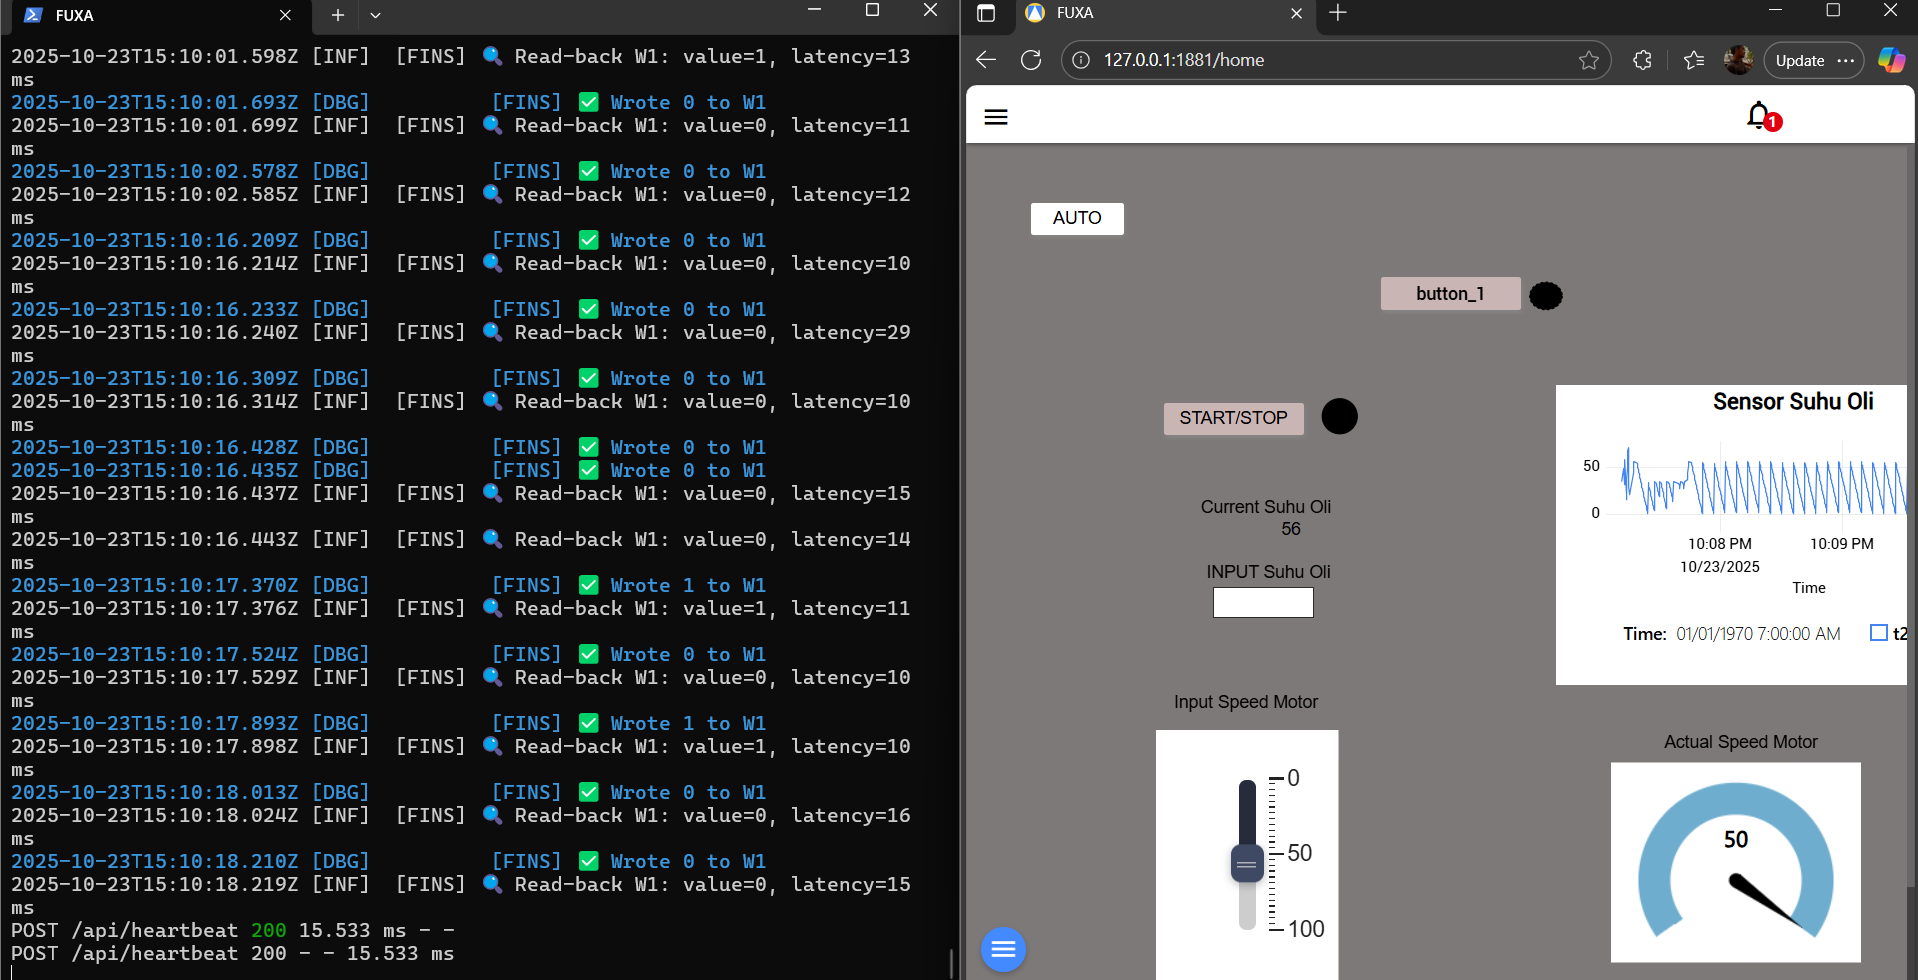
\includegraphics[width=\textwidth]{images/test_latensi.png}
    \caption{Tampilan log hasil pengujian latensi baca/tulis FINS antara FUXA dan PLC Omron}
    \label{fig:test-latensi}
\end{figure}

Berdasarkan hasil pengujian pada Gambar~\ref{fig:test-latensi}, diperoleh waktu latensi baca/tulis rata-rata sebesar \textbf{12~ms}. Nilai ini menunjukkan bahwa sistem mampu merespons perubahan input dari pengguna dengan cepat, berada jauh di bawah target KPI sebesar 200~ms. Dengan demikian, performa komunikasi antara HMI dan PLC dapat dikategorikan OK.

 

\subsubsection{Persentase Sukses Komunikasi}
\label{sec:persentase-sukses}

Pengujian persentase sukses komunikasi dijalankan menggunakan skrip Node.js yang mengirimkan permintaan membaca (\textit{read request}) berulang ke alamat memori \texttt{D100} pada PLC. Pengujian memiliki parameter utama sebagai berikut:
\begin{itemize}
\item Jumlah permintaan total: 1000 request.
\item Tingkat konkurensi: 10 request paralel (concurrency = 10).
\item Transport: FINS over UDP pada port 9600 (sesuai konfigurasi uji).
\item Kriteria respons dianggap \emph{berhasil}: diterimanya paket balasan dari PLC yang menunjukkan \texttt{Response Code 0000} dan Service ID yang sesuai.
\item Kegagalan dicatat jika tidak ada respons (timeout) atau respons berisi kode kesalahan/format tidak sesuai dalam batas waktu yang ditentukan oleh skrip pengujian.
\item Semua event (success/fail/timeout) dicatat ke log terminal untuk analisis pascauji.
\end{itemize}

Pengujian dijalankan oleh skrip yang memulai 10 worker paralel; setiap worker mengirimkan permintaan baca berurutan ke alamat \texttt{D100} sampai jumlah permintaan gabungan mencapai 1000. Untuk setiap permintaan skrip menunggu balasan hingga batas waktu yang ditetapkan. Jika balasan diterima dengan \texttt{Response Code = 0000} permintaan dicatat sebagai berhasil, jika tidak maka permintaan dicatat gagal. Setelah semua 1000 permintaan selesai, skrip menghitung jumlah sukses, jumlah gagal, dan persentase sukses, serta menyimpan log dan tangkapan paket Wireshark untuk analisis akar penyebab kegagalan.

Hasil pengujian menunjukkan \textbf{990 request berhasil} dari \textbf{1000 request total} (dapat dilihat di Gambar~\ref{fig:hasil-sukses-komunikasi}), sehingga diperoleh \textbf{persentase sukses 99\%}, melampaui target KPI minimal sebesar 95\%. Analisis log dan capture paket mengungkapkan hal berikut:
\begin{itemize}
\item Dari 10 kegagalan, mayoritas tercatat sebagai \textbf{timeout}. Timeout ini terekam juga pada Wireshark sebagai paket request tanpa paket reply yang sesuai.
\item Tidak ada indikasi kesalahan framing FINS yang sistemik (Gambar~\ref{fig:capture-wireshark} menunjukkan \texttt{Response Code 0000} pada paket yang sukses).
\item Faktor penyebab kegagalan yang mungkin: kehilangan paket UDP di jaringan fisik/layer link, sementara PLC sedang sibuk memproses permintaan lain (antrian internal), atau packet scheduling pada host yang mengirim request terlalu agresif untuk kondisi jaringan uji.
\end{itemize}

\begin{figure}[H]
    \centering
    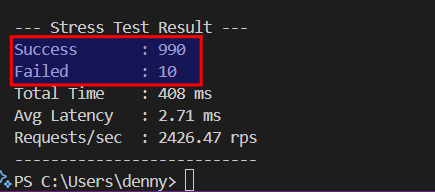
\includegraphics[width=\textwidth]{images/hasil_success_rate.png}
    \caption{Tampilan log hasil pengujian persentase sukses komunikas}
    \label{fig:hasil-sukses-komunikasi}
\end{figure}

\subsubsection{Penggunaan CPU dan Memori Server}
Selama pengujian performa, pemantauan dilakukan melalui \textit{Task Manager} pada sistem operasi Windows untuk memisahkan beban proses antara \textbf{frontend} dan \textbf{backend}. 
Gambar~\ref{fig:cpu-mem-usage} memperlihatkan bahwa proses \textbf{Microsoft Edge} mewakili bagian \textit{frontend} (aplikasi HMI berbasis Angular yang berjalan di browser), sedangkan proses \textbf{Node.js JavaScript Runtime} mewakili bagian \textit{backend} (server FUXA yang menjalankan konektor FINS).

\begin{figure}[H]
    \centering
    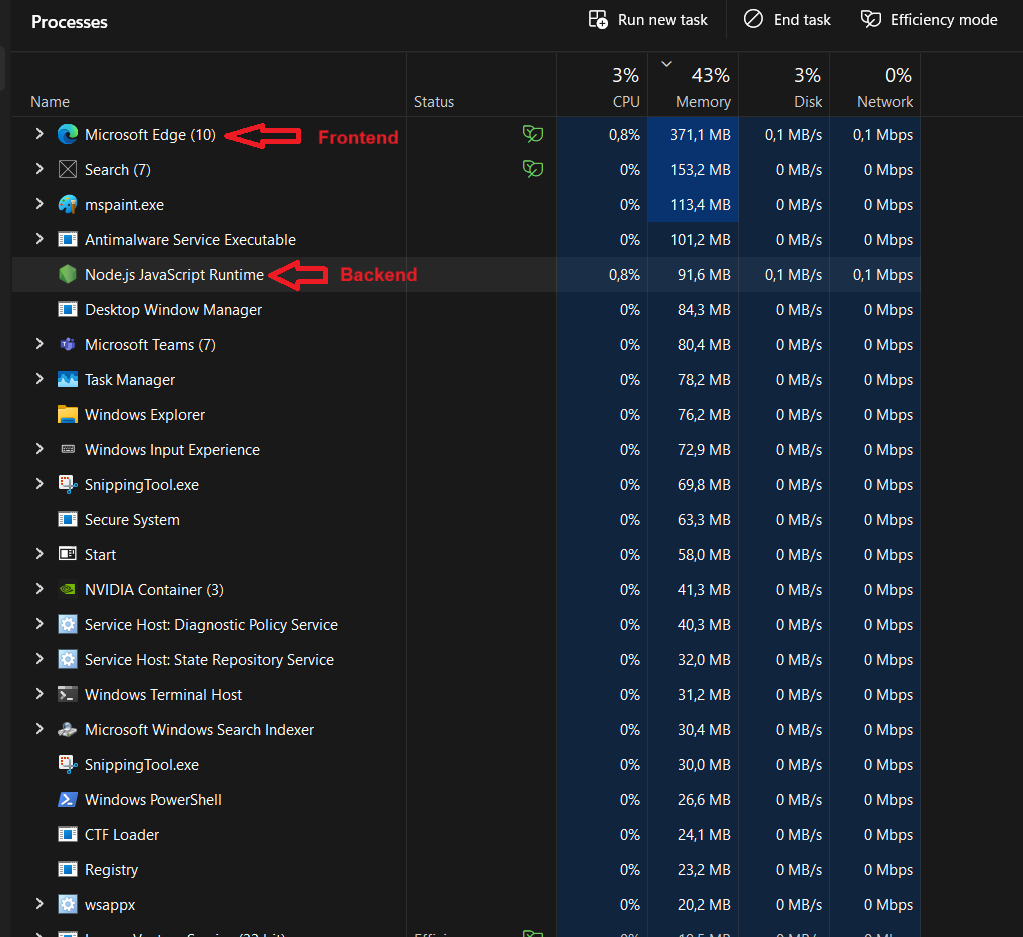
\includegraphics[width=0.85\textwidth]{images/cpu and mem usage.png}
    \caption{Pemantauan penggunaan CPU dan memori oleh frontend (Edge) dan backend (Node.js)}
    \label{fig:cpu-mem-usage}
\end{figure}

Selama uji beban berlangsung, total penggunaan CPU berada pada kisaran rata-rata \textbf{3\%} secara keseluruhan, 
dengan kontribusi sekitar \textbf{0.8\%} dari proses \textit{Node.js backend} dan \textbf{0.8\%} dari proses \textit{frontend browser}. 
Rata-rata konsumsi memori tercatat sebesar \textbf{91 MB} untuk backend dan sekitar \textbf{371 MB} untuk frontend browser.  

Nilai tersebut masih jauh di bawah batas KPI yang telah ditetapkan, yaitu maksimum \textbf{30\% penggunaan CPU} dan \textbf{500 MB penggunaan memori server}. 
Hal ini menunjukkan bahwa arsitektur HMI berbasis Node.js dan Angular mampu beroperasi dengan efisien tanpa membebani sumber daya sistem secara berlebihan.


\subsubsection{Waktu Deteksi Alarm}
Waktu deteksi alarm dihitung sejak kondisi yang memicu alarm terpenuhi hingga indikator alarm muncul di antarmuka pengguna.  
Waktu deteksi adalah sekitar 1000 ms, jauh lebih lambat dari batas KPI 200 ms. Hal ini dikarenakan interval terkecil sistem HMI untuk mendeteksi situasi dan kemudian mengirimkan alarm adalah 1 detik seperti yang ditunjukkan pada gambar~\ref{fig:alarm-interval}. 

\begin{figure}[H]
    \centering
    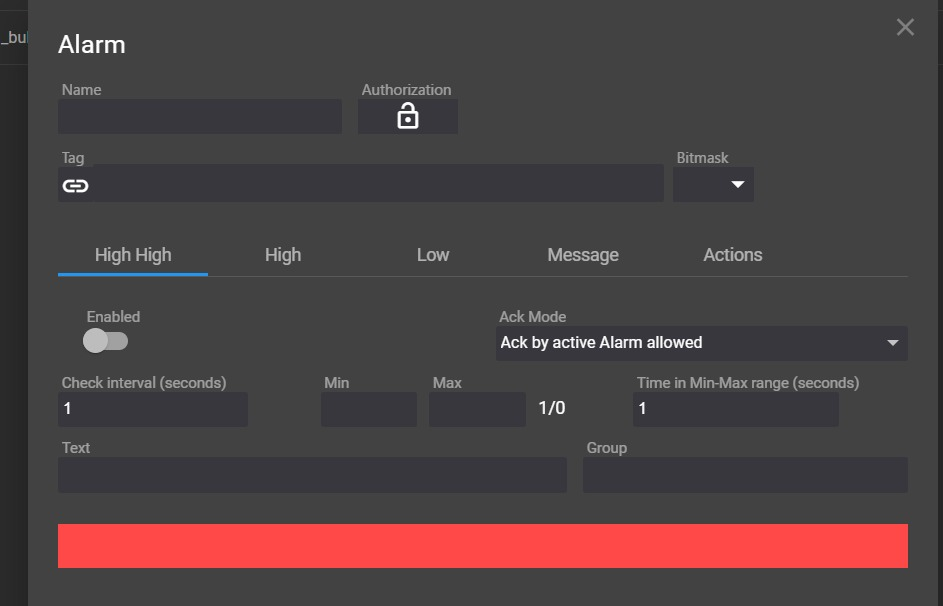
\includegraphics[width=0.8\textwidth]{images/alarm_interval.jpeg}
    \caption{Batasan interval waktu deteksi alarm sistem HMI}
    \label{fig:alarm-interval}
\end{figure}

\subsubsection{Waktu Mulai Aplikasi}
Aplikasi diuji untuk mengetahui waktu yang dibutuhkan sejak proses inisialisasi hingga tampilan utama siap digunakan.  
Rata-rata waktu mulai aplikasi adalah 3,14 detik, memenuhi KPI $\leq$ 10 detik.

\begin{figure}[H]
    \centering
    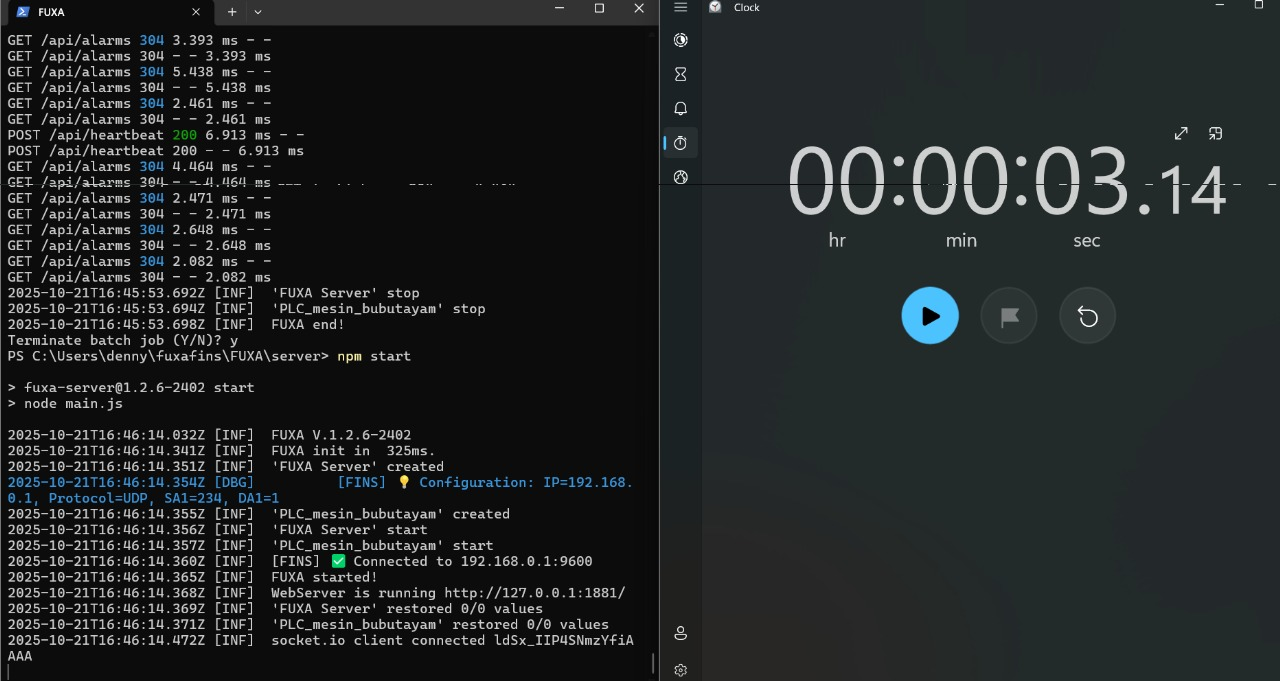
\includegraphics[width=0.8\textwidth]{images/starting_time.jpeg}
    \caption{Tangkapan layar proses inisialisasi aplikasi}
    \label{fig:startup-time}
\end{figure}

\subsection{Observasi Fault Tolerance}
\begin{itemize}
    \item Saat kabel dicabut, modul mendeteksi timeout dan mengirimkan event \texttt{device-status:changed} dengan status \texttt{connect-error} (UI merah). 
    \item Mekanisme reconnect otomatis dijalankan setiap 3--5 detik. Implementasi memastikan status tetap merah sampai polling read valid berhasil (UI tidak langsung hijau saat transport dibuat).
\end{itemize}



\subsection{Evaluasi Berbasis Responden}
Evaluasi dilakukan terhadap 10 responden (operator dan teknisi) dengan menggunakan kuesioner skala Likert 1--5. Lima aspek utama yang dinilai meliputi kemudahan konfigurasi, kejelasan tampilan nilai dan status, responsivitas sistem, konsistensi UI, serta kepuasan umum terhadap integrasi FINS pada FUXA.

\subsubsection{Data Mentah Kuesioner}
Tabel berikut menyajikan data mentah dari 10 responden. Untuk menjaga konsistensi penamaan, setiap responden diberi kode R1 hingga R10.

\begin{table}[H]
\centering
\begin{tabular}{|c|p{2.2cm}|p{2.5cm}|p{2.5cm}|p{2.2cm}|p{2cm}|}
\hline
\textbf{Responden} & \textbf{Kemudahan} & \textbf{Kejelasan Status} & \textbf{Responsivitas} & \textbf{Konsistensi UI} & \textbf{Kepuasan Umum} \\ \hline
R1 & 4 & 4 & 5 & 4 & 4 \\ \hline
R2 & 5 & 4 & 4 & 4 & 5 \\ \hline
R3 & 5 & 4 & 4 & 4 & 5 \\ \hline
R4 & 4 & 4 & 4 & 4 & 4 \\ \hline
R5 & 4 & 4 & 4 & 4 & 4 \\ \hline
R6 & 4 & 5 & 4 & 4 & 4 \\ \hline
R7 & 4 & 4 & 5 & 4 & 4 \\ \hline
R8 & 4 & 4 & 4 & 4 & 4 \\ \hline
R9 & 4 & 4 & 5 & 4 & 5 \\ \hline
R10 & 4 & 4 & 4 & 4 & 4 \\ \hline
\rowcolor{gray!20}
\textbf{Rata-rata} & \textbf{4.2} & \textbf{4.1} & \textbf{4.3} & \textbf{4.0} & \textbf{4.3} \\ \hline
\end{tabular}
\caption{Data hasil evaluasi responden (R1--R10) beserta rata-rata}
\label{tab:raw-respondent}
\end{table}

\subsubsection{Ringkasan Hasil Evaluasi}
Rata-rata skor tiap aspek dihitung dari data mentah pada Tabel~\ref{tab:raw-respondent}. Ringkasan hasilnya ditunjukkan pada tabel berikut:

\begin{table}[H]
    \centering
    \begin{tabular}{|c|c|p{3.5cm}|}
        \hline
        \textbf{Aspek} & \textbf{Rata-rata Skor} & \textbf{Interpretasi} \\ \hline
        Kemudahan konfigurasi & 4.2 & Baik \\ \hline
        Kejelasan tampilan nilai dan status & 4.1 & Baik \\ \hline
        Responsivitas (persepsi operator) & 4.3 & Sangat baik (perubahan terlihat instan) \\ \hline
        Konsistensi UI dengan protokol lain & 4.0 & Baik \\ \hline
        Kepuasan umum & 4.3 & Puas \\ \hline
    \end{tabular}
    \caption{Ringkasan hasil evaluasi berbasis responden}
    \label{tab:usability}
\end{table}

Komentar kualitatif utama:
\begin{itemize}
    \item Operator menyukai indikator status koneksi yang jelas (merah/kuning/hijau).
    \item Beberapa responden meminta tombol \textit{Check Connection} yang lebih menonjol untuk verifikasi manual.
    \item Disarankan menambahkan mode logging ringkas untuk troubleshooting non-teknis.
\end{itemize}

\subsection{Pembahasan Singkat}
\begin{itemize}
    \item Implementasi berhasil menyediakan HMI yang responsif dan fungsional untuk operasi baca/tulis terhadap PLC Omron melalui FINS pada skenario lab.
    \item Mekanisme reconnect dan alarm bekerja sesuai rancangan; penting untuk menghindari men-set status hijau sampai polling valid berhasil — hal ini sudah diterapkan.
    \item Area perbaikan: optimasi polling scheduler pada beban sangat tinggi, pembersihan listener untuk mencegah memory leak jangka panjang, dan dokumentasi lebih rinci untuk operator non-teknis.
\end{itemize}

